\documentclass[a4j,twocolumn]{ltjarticle}

%ページ設定
\setlength{\topmargin}{-10mm}
\setlength{\oddsidemargin}{-5mm}
\setlength{\evensidemargin}{-5mm}

\setlength{\textheight}{230mm}
\setlength{\textwidth}{170mm}
\setlength{\columnsep}{10mm}%コラムとコラムの間.よってコラムの横幅は(texwidth-columnsep)/2
\setlength{\footskip}{15mm}
%パッケージ
\usepackage{graphicx,color}
\usepackage{bm}
\usepackage{amsmath}
\usepackage{amsfonts}

%数学関数
\newcommand{\B}[1]{\bm #1} 
\newcommand{\s}[2]{{#1}\cdot{#2}} 
\newcommand{\R}{\mathbb{R}}
\newcommand{\M}{\mathbb{M}}
\newcommand{\df}[2]{\displaystyle{\frac{#1}{#2}}}
\newcommand{\qed}{
\begin{flushright}
\vspace{-8mm}
$\Box$
\end{flushright}
}

%ミニセクション
\newcommand{\minisection}[2]{\flushleft{\bf (#1)#2}\\ \ \ \ }

%図,表の名前変更
\renewcommand{\figurename}{Fig.}
\renewcommand{\tablename}{Tab.}

% refの拡張
\newcommand{\reffig}[1]{\figurename \ref{#1}}
\newcommand{\refeq}[1]{式(\ref{#1})}
\newcommand{\reftab}[1]{\tablename \ref{#1}}

% 図
\newcommand{\includefigure}[3]{
\begin{center}
\includegraphics[width=80mm]{#1}
\caption{#2}
\label{#3}
\end{center}
}
% 図 widthを変更したいときはこっち
\newcommand{\includefigurewidth}[4]{
\begin{center}
\includegraphics[width=#2]{#1}
\caption{#3}
\label{#4}
\end{center}
}

\usepackage{setspace} % setspaceパッケージのインクルード
\usepackage{enumitem}
\usepackage{graphicx}
%「Weekly Report」 
\newcommand{\Weekly}[5]{
\twocolumn[
 \begin{center}
  \bf
 第 #1 回 Weekly Report\\
 \huge
深層学習を用いた動画像からの危険認知手法のための基礎的研究\\

 \end{center}
 \begin{flushright}
  #2 月\ \ \  #3 日 \ \ \ #4 \\\
  #5
 \end{flushright}
]
}
%\setstretch{0.5} % ページ全体の行間を設定

\begin{document}

\Weekly{6}{5}{12}{(火)}{\ 小松 大起}

\section{PredNet}
PredNet は Deep Recurrent Convolutional Neural Network  の 1 種で 神経科学の概念である Predictive Coding を組み込んで作られたモデルである.

\subsection{Predictive Coding}

\begin{figure}[hb]
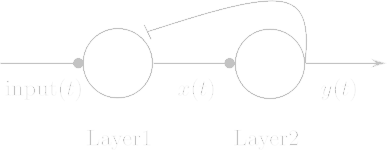
\includegraphics[scale=0.5]{predictivecoding.png}
 \caption{2 つのニューロンの模式図}
 \end{figure}

2 種類のニューロンが存在するとし,それを図 1 で示す.
図の上では 2 つのニューロンであるが, Layer1 と Layer2 という 2 層について,それぞれを代表するニューロンを 1 つずつ描いている.
まず, Layer1 のニューロンは下層から
$input(t)$
を受け取る.
これは入力刺激と呼ばれる.
次に Layer1 のニューロンは
$x(t)$
を出力する.
これは誤差信号または残差と呼ばれ,以下の式が成り立つ.
%%%%%%%%%%%%%%%
\begin{equation}
x(t) = input(t) - y(t)
\end{equation}
%%%%%%%%%%%%%%%
また, $y(t)$ は Layer2 のニューロンからの出力で, Layer1 のニューロンへの入力を予測する.ここで
%%%%%%%%%%%%%%%
\begin{equation}
dy/dt = x(t) = input(t) - y(t)
\end{equation}
%%%%%%%%%%%%%%%
であり,$dy/dt = 0$ すなわち $y(t) = input(t)$ となるように学習が進行するモデルである.

\subsection{PredNet の層構造}
PredNet の各層には 4 つの素子が存在しておりそれぞれ、Target, Representation, Prediction, Errorと呼ぶ.
Target は下層からの出力である誤差信号をエンコード,符号化する.
Representation は Recurrent unitで,上層からの出力,側方からの誤差信号, 1 ステップ前の自分の出力を受け取る.
Representation unit は Target の予測をする Prediction unit に投射し,入力の予測が出力される.
Error は Prediction と Target の誤差であり, Error は上層に送られる.
この Error が小さくなるように学習を進めていく.
また,層構造の例を図 2 に示す.

 \begin{figure}[hb]
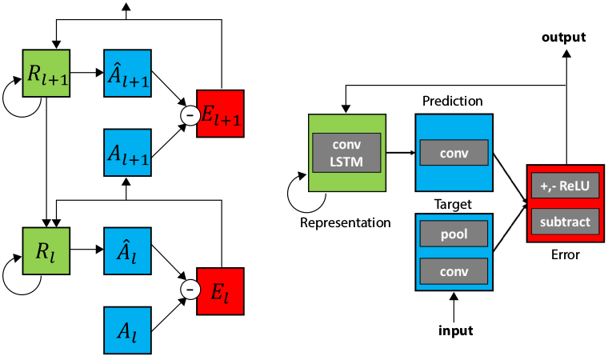
\includegraphics[scale=0.4]{prednet.png}
 \caption{PredNet の層構造の例}
\end{figure}

\section{使用した動画像}
\subsection{lyft level5}
lyft という団体が公開しているデータセット. lyft level5 が 2 年間にわたって収集してきた.

\section{先週までの作業}
\begin{itemize}
          \item PredNet について
          \item 
\end{itemize}

\section{今週の作業}
\begin{itemize}
         \item PredNet のサンプルコードを現在のバージョンの python3.7.3 で使えるように整形中.また,そのコードは kitti というデータセット使用することが前提なので他の動画でできるか試してみる.
         \item ゼミの予習
\end{itemize}

\section{来週以降の作業}
\begin{itemize}
         \item lyft level5 でサンプルコードを動かせるようにする.
\end{itemize}




\end{document}
